\documentclass[french, a4paper, 12pt, openany]{report}
% General packages
\usepackage{amsfonts, amssymb, amsthm}
\usepackage{array}
\usepackage{enumitem}
\usepackage{mathtools}
\usepackage{stmaryrd}
\usepackage{empheq, environ} % packages for system environment
\usepackage{calrsfs} % better mathcal letters
\usepackage{graphicx}


% Layout
\usepackage{fancyhdr, fancyvrb}
\usepackage{lastpage}
\usepackage[left=2.0cm, right=2.0cm, top = 2.0cm, bottom = 2.0cm]{geometry}
\usepackage{lettrine, yfonts}
\usepackage{multicol}
\usepackage{minitoc}
\usepackage{hyperref}
\hypersetup{hyperindex=true, colorlinks, linkcolor=blue, urlcolor=blue, citecolor=blue, breaklinks=true}
\everymath{\displaystyle}


% Language
\usepackage[utf8]{inputenc}
\usepackage[T1]{fontenc}
\usepackage{babel}


% Minted
\newcommand{\python}{\mintinline[breaklines=true, breakanywhere=true]{python}}
\newminted{python}{
	linenos=true,
	tabsize=4,
	breaklines=true,
	fontfamily=courier,
	autogobble,
	style=rainbow_dash,
	xleftmargin=5pt,
	xrightmargin=5pt,
	frame=lines
}


% Pagestyle
\everymath{\displaystyle}
\pagestyle{fancy}
\fancypagestyle{plain}


% Customs commands and environnements
\renewcommand{\leq}{\leqslant}
\renewcommand{\geq}{\geqslant}
\renewcommand{\ker}{\mathrm{Ker\,}}
\renewcommand{\vec}{\overrightarrow}
\newcommand{\im}{\mathrm{Im\,}}
\newcommand{\derivative}[2]{\frac{\mathrm{d} #1}{\mathrm{d}#2}}
\newcommand{\enluminure}[2]{\lettrine[lines=3]{\small \initfamily #1}{#2}}
\newcommand{\nnchapter}[1]{
	\chapter*{#1}
	\addstarredchapter{#1}
	\markboth{\uppercase{#1}}{}		
}

\def\restriction#1#2{\mathchoice
              {\setbox1\hbox{${\displaystyle #1}_{\scriptstyle #2}$}
              \restrictionaux{#1}{#2}}
              {\setbox1\hbox{${\textstyle #1}_{\scriptstyle #2}$}
              \restrictionaux{#1}{#2}}
              {\setbox1\hbox{${\scriptstyle #1}_{\scriptscriptstyle #2}$}
              \restrictionaux{#1}{#2}}
              {\setbox1\hbox{${\scriptscriptstyle #1}_{\scriptscriptstyle #2}$}
              \restrictionaux{#1}{#2}}}
\def\restrictionaux#1#2{{#1\,\smash{\vrule height .8\ht1 depth .85\dp1}}_{\,#2}}

\NewEnviron{system}[1][2]
{
	\begin{empheq}[left=\empheqlbrace]{alignat=#1}
        \BODY
    \end{empheq}
}
\NewEnviron{subsystem}[1][2]
{ 
    \begin{subequations}
    \begin{empheq}[left=\empheqlbrace]{alignat=#1}
    	\BODY
    \end{empheq}
    \end{subequations}
}
   
\newtheorem{theoreme}{Théorème}[section]
\newtheorem{definition}[theoreme]{Définition}
\newtheorem{proposition}[theoreme]{Proposition}
\newtheorem{propriete}[theoreme]{Propriété}
\newtheorem{lemme}[theoreme]{Lemme}
\newtheorem{formule}[theoreme]{Formule}
\newtheorem{remarque}[theoreme]{Remarque}
\newtheorem{exemple}[theoreme]{Exemple}

\usepackage{titling}
\usepackage{graphicx}


\title{\sc Modèle de Vicsek}
\author{Alexis Peyroutet, Antoine Royer}
\date{Janvier – Juin 2023}

\lhead{}
\rhead{\thetitle}
\lfoot{\theauthor}
\cfoot{\thepage\ $|$ \pageref{LastPage}}
\rfoot{L3 PCAME\\2022 — 2023}

\renewcommand{\headrulewidth}{0.4pt}
\renewcommand{\footrulewidth}{0.4pt}




\begin{document}
\makeatletter
\begin{titlepage}
	\centering
	
	
\includegraphics[width=8cm]{images/ut3.png} \hfill 
\includegraphics[width=8cm]{images/uppa.png} \\
	{\large{\sc Licence 3 de Physique, Chimie, Astrophysique, Météorologie et Énergie}} \\
	\rule{0.5\linewidth}{0.4pt} \\
	{\sc Rapport du projet numérique} \\
	
	%\rule{\linewidth}{0.4pt}
	
	\vfill
	{\huge {\sc \@title}} \\ \vspace{1cm}
	{\Large \@author} \\
	
	\vfill 
	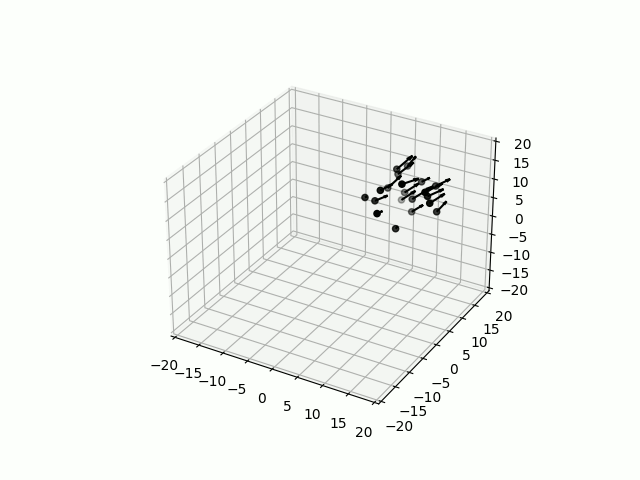
\includegraphics[width=0.7\linewidth]{images/page_garde2.png}
	\vfill
	{\Large \@date}
	\rule{\linewidth}{0.4pt}
\end{titlepage}
\makeatother

\tableofcontents

\nnchapter{Introduction}


	Notre sujet est intitulé «~Modèle de Vicsek~». Le but de ce projet numérique est de reproduire de manière numérique le modèle de Vicsek.

	Le modèle de Vicsek a été crée par le scientifique Tamás Vicsek. Il s'agit d'un physicien hongrois connu pour ses contributions à la physique statistique, à la biologie et à la dynamique des systèmes. Il est né le 10 mai 1948 (~74 ans~) à Budapest. Il est aujourd'hui professeur à l'Université Eötvös Loránd de Budapest. Ce brillant physicien est d'ailleurs un des membres de l'Académie hongroise des sciences et a reçu de nombreux prix pour ses contributions à la physique, notamment le prix Széchenyi (~1999~) ou encore le prix Lars Onsager (~2020~).

	Mais Tamás Vicsek est surtout connu pour son travail sur les systèmes auto-organisés, qui étudient les mouvements collectifs. Il a ainsi travaillé sur le comportement d'agents individuels qui interagissent avec d'autres agents aux alentours, ses observations montrent que des motifs de mouvements collectifs emmergent d'eux-même. Le groupe se déplace alors de manière coordonnée sans qu'il n'y ait de leader comme on peut l'observer notamment dans la migration des grues. Nous pouvons citer comme exemples~: les bancs de poissons, les regroupements de certains oiseaux, les essaims d'insectes, ou encore le mouvement de foules.

	 Le premier modèle de Vicsek voit ainsi le jour en 1995.\\
	 
	
\chapter{Présentation et explications}	

	Le modèle de Vicsek permet d'étudier un groupe d'agents qui se déplace dans un espace. Chacun des agents a une vitesse donnée (~en norme et en direction~). Chaque agent va interagir avec ses voisins, ce qui concrètement se traduit par des changements concernant la norme et la direction de la vitesse. Nous allons alors observer la création d'un mouvement de groupe du aux interactions entre les agents. Cependant, les agents observables dans la vie réelle ne suivent pas toujours le groupe à la perfection, et il peut arriver qu'un agent s'écarte, de manière aléatoire, des autres. C'est pour cela que Vicsek a introduit une notion de bruit dans son modèle. En effet, à chaque pas de temps, chaque agent va prendre la direction moyenne des agents autour de lui et à cette direction va venir se superposer un bruit qui le fera peut-être dévier dans une autre direction. En augmentant significativement le bruit, le groupe pert son mouvement collectif et les agents prennent alors des directions aléatoires.\\

	Le modèle de Vicsek s'implémente très simplement puisqu'il se réduit à deux équations~:
	\[
		\Theta_{i}(t+dt) = \Theta_{j |r_{i}-r_{j}|<r} + \eta_{i}(t)
	\]
	\[
		r_{i}(t+dt) = r_{i}(t) + v_{i}\Delta t
	\]
	dans lesquelles $r_{i}$ la position de chaque individu donnée par un vecteur de position, nous prendrons $i$ comme indice de l'agent en question et $t$ le temps. Nous noterons également $\eta$ le bruit et $\Theta$ pour l’angle définissant la direction de sa vitesse. Ici, $\Theta_{j |r_{i}-r_{j}|<r}$ nous indiquera la direction moyenne des vitesses des agents dans un cercle de rayon $r$. L'indice $j$ repésentera alors l'ensemble des voisins de $i$ compris dans ce cercle.\\

	Ce qui est intéressant, c'est que nous pouvons, en modifiant certains paramètres du système étudié, observer un mouvement de foule plus fort ou plus faible. Nous pourrons alors jouer sur la surface et les dimensions du plan étudié, le nombre d'agent et donc par conséquent la densité de population et même le bruit.\\

	Le modèle de Vicsek est important pour étudier le comportement de certains animaux en biologie ou encore l'étude des foules. Ce modèle peut même être utile à la construction de bâtiment. En effet, le comportement des foules peut être intéressant dans la conception d'entrées et de sorties d'un espace fermé, notamment dans un moment de panique. La foule va s'éloigner du danger est emprunter les sorties. Il est alors crucial de prévoir le comportement des agents pour placer les sorties de manière à ce que le débit d'agent sortant soit le plus important possible.\\
	
	Nous pouvons également retrouver le modèle de Vicsek dans la robotique. C'est un précieux outil pour la technologie du monde moderne. Il peut être utiliser dans des programmes informatiques qui gèrent le déplacement de systèmes de robots (~comme les drones~).\\ 

	C'est avec tout cela que nous essayerons, à travers ce projet, de reproduire numériquement des mouvements collectifs et ainsi étudier le modèle de Vicsek.
	
\chapter{Méthode employée}
\section{Classes et méthodes}

    Pour ce projet, la programmation orientée objet s'est naturellement imposée. Nous utilisons ainsi deux classes principales appelées \verb|Agent| et \verb|Group| qui fixent respectivement les paramètres de l'agent et du groupe. Assez simplement, la classe \verb|Group| contient une liste d'instances de la classe \verb|Agent| et permet de les représenter dans l'espace et le temps. La classe \verb|Agent| permet d'encapsuler toutes les données de chaque agent~: position, vitesse et direction.
    
   Ainsi, nous pouvons retrouver dans chaque classe, plusieurs méthodes qui vont nous aider à mieux définir les groupes et les agents. \\
   
\section{Premiers pas sur le code}
   
   Nous avons tout d'abord codé les premières méthodes qui servirons à initialiser les différents paramètres des agents ou du groupe. Par exemple, la fonction \verb|__init__|  énumère une liste d'instances qui nous renseignerons sur la vitesse, la position, le bruit.\\
   Nous nous servons également de méthodes pour éviter toute incohérence avec le modèle (~mais au contraire respecter les deux équations~). Nous pourrons notamment éviter de retrouver deux agents avec les mêmes coordonnées.\\
   
   Après avoir crée notre groupe avec \verb|group_generator|, nous utilisions dans un premier temps la méthode  \verb|compute_figure| qui nous crée une image sur un espace dont nous fixions les dimensions. Nous obtenions un fichier PNG que nous pourrons visualiser et étudier grâce à \verb|run|.\\
	
	Ce premier abord du modèle, nous permettait déjà d'observer plusieurs images d'un groupe dans un espace. Notre fonction \verb|compute_figure| permettait déjà d'obtenir un nombre d'images en deux ou trois dimensions.Nous obtenions déjà des images comme celles-ci~:\\
	
	\begin{figure}[!h]
		\centering
		\begin{tabular}{cc}
			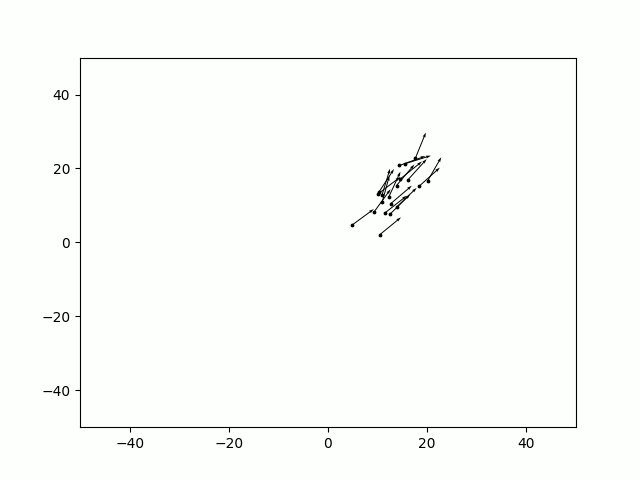
\includegraphics[width=8cm]{images/image_2.png} & 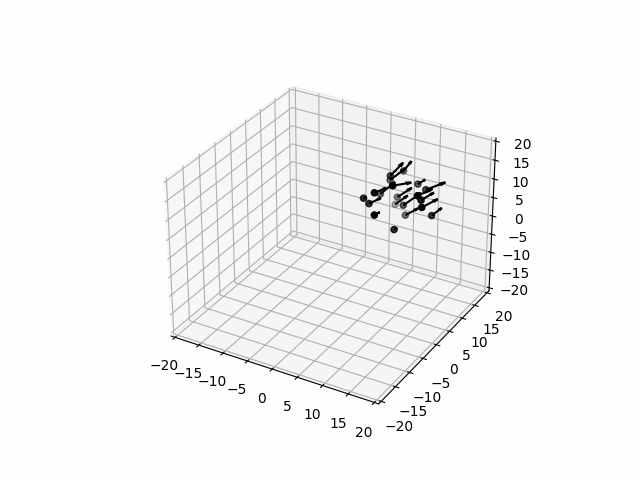
\includegraphics[width=10cm]{images/image_1.png} \\
		\end{tabular}
		\caption{Premières images obtenues en 2D et 3D }
	\end{figure} 

\section{Premiers résultats et interprétation physique}

   Pour pouvoir observer un mouvement, il est plus utile de regarder une vidéo que des images. Nous avons alors créer notre première fonction \verb|compute_animation| qui utilise la fonction \verb|Artist_animation| matplotlib.pyplot. Nous arrivions alors à générer des fichiers GIF avec le nombre de frames souhaité.
   
   Après avoir généré plusieurs animations avec des groupes de tailles différentes. Nous avons pu déjà tirer quelques conclusions. En effet, nous observions des mouvements de groupes. Les agents qui avaient des positions de départ aléatoires, sont influencés les uns les autres selon la distance avec leurs voisins. On observe d'ailleurs des mouvements collectifs plus importants quand la densité d'agent est plus forte. En revanche, quand les agents sont moins nombreux dans un même espace, nous observons davantage de formations de petits groupes ou des agents solitaires. 
   
   
	\begin{figure}[!h]
		\centering
		\begin{tabular}{cc}
			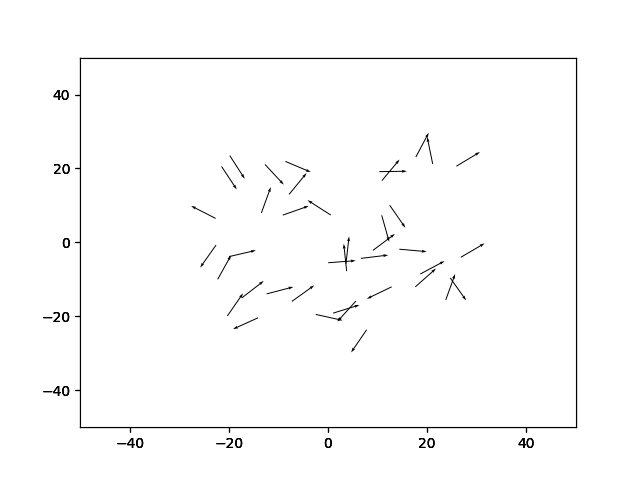
\includegraphics[width=8cm]{images/image_3.png} & 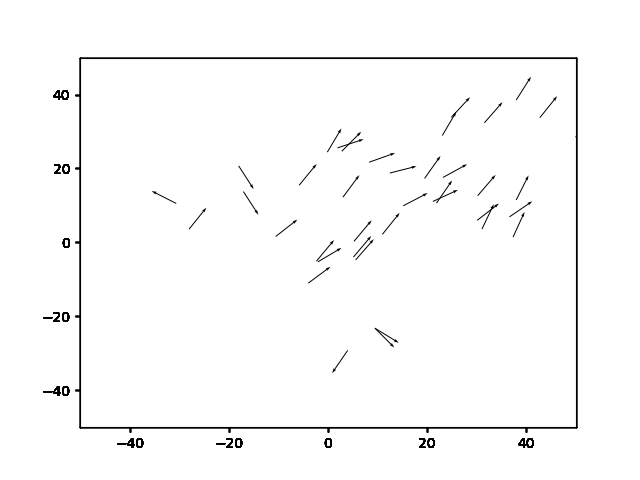
\includegraphics[width=8cm]{images/image_4.png} \\
		\end{tabular}
		\caption{Début et fin d'une animation 2D}
	\end{figure} 
   
   
\section{Mouvements de groupe}

   Pour mieux observer les mouvements de groupe, nous avons décidé de mettre une couleur à nos agents selon la direction qu'il vont prendre. Cela permet de mieux visuliser les différents groupe et d'enlever les flèches qui pouvont être un peu gênantes pour bien discerner le mouvement collectif. Nous avons employé cette méthode pour tout le reste du projet.
   
   \begin{figure}[!h]
		\centering
		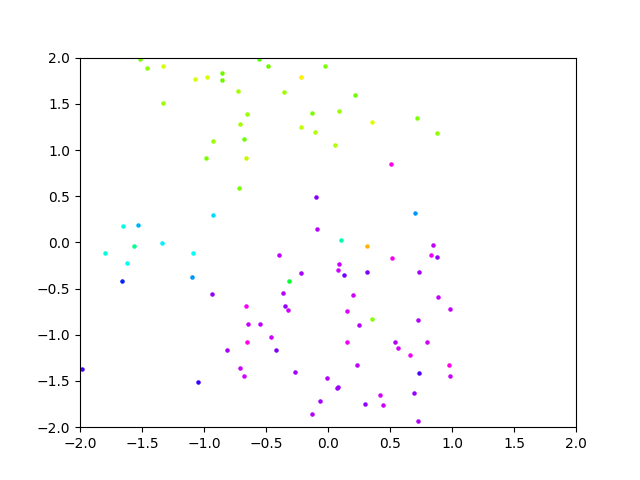
\includegraphics[width=10cm]{images/image_6.png}
		\caption{Image colorée pour la visualisation de groupe}
		\label{couleurs_image}
	\end{figure}  
   
   Sur cette nouvelle figure \ref{couleurs_image}, nous voyons bien les différents groupe crées. Sur l'image de droite, on discerne trois groupe principaux en violet,vert et cyan. On distingue encore mieux les mouvements lors de l'animation.
   
   Nous avons d'ailleurs pu observer une organisation intéréssante des agents sur certaines animations. En effet, les agents se regroupent premièrement en plusieurs petits groupes. Enfin, les petits groupes s'unissent pour former un seul et même grand groupe.
   
    \begin{figure}[!h]
		\centering
		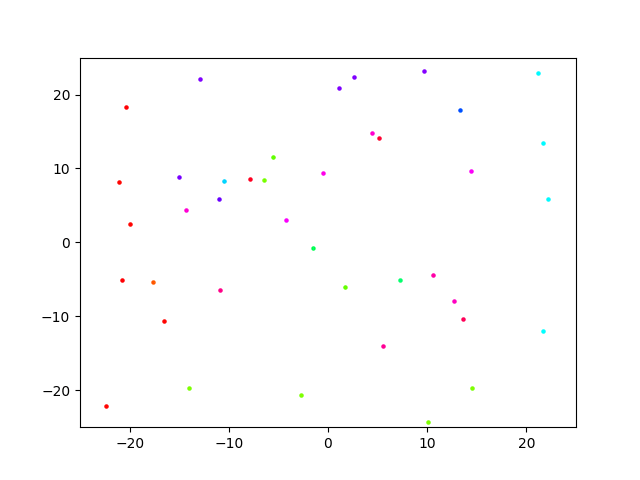
\includegraphics[width=10cm]{images/image_8.png}
		\caption{Image de départ }
		\label{couleurs_image}
	\end{figure} 
	
   \begin{figure}[!h]
		\centering
		\begin{tabular}{cc}
			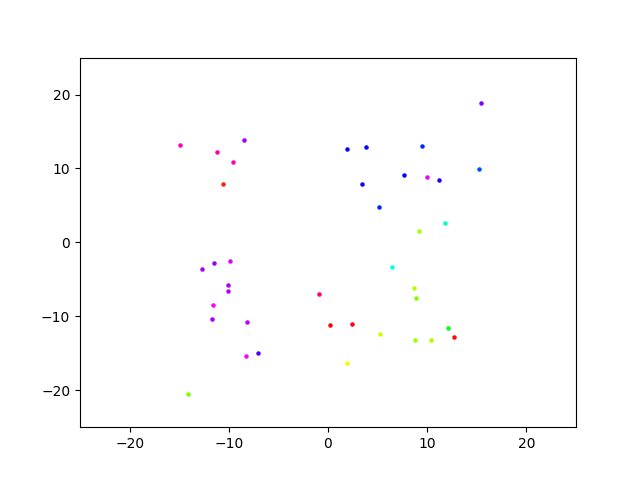
\includegraphics[width=10cm]{images/image_7.png} & 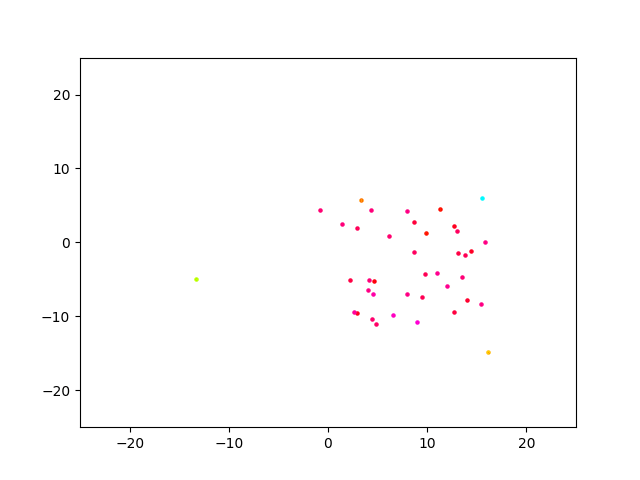
\includegraphics[width=10cm]{images/image_9.png} \\
		\end{tabular}
		\caption{Formations de petits groupe puis d'un seul et même groupe}
	\end{figure} 
	
	Ceci montre encore un fois très bien l'influence entre les agents.
\newpage
\section{Paramètre de bruit}
   
   
   Nous avons déjà pu observer l'impact du bruit sur les populations. Nous voyons alors que ce paramètre est capital pour l'observation de mouvements collectifs. Si celui-ci est trop fort, les agents feront route seul et ne s'occuperont pas du tout du mouvement des voisins. En revnache, les mouvements collectifs seront davantages présents avec un bruit qui tend vers zéro.

Par exemple, en regardant ces images~:


   
	\begin{figure}[!h]
		\centering
		\begin{tabular}{cc}
			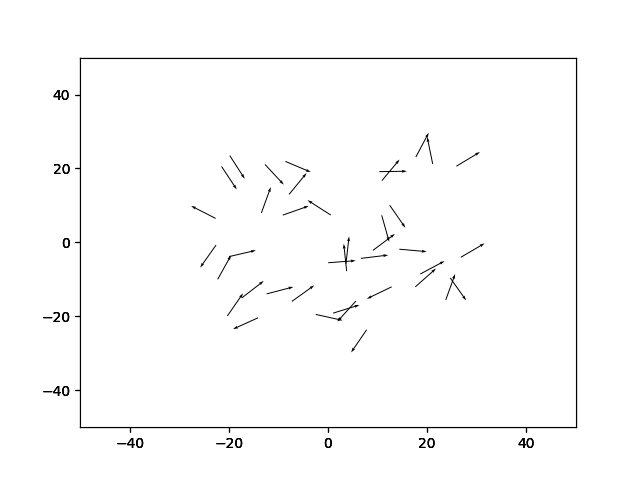
\includegraphics[width=8cm]{images/image_3.png} & 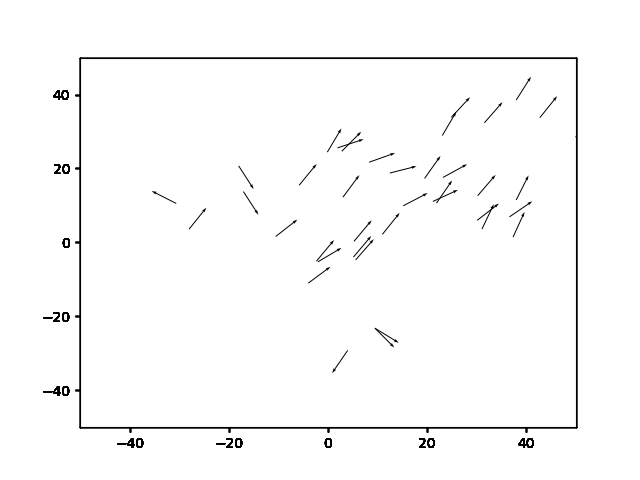
\includegraphics[width=8cm]{images/image_4.png} \\
		\end{tabular}
		\caption{Visualisation de l'impact du bruit}
	\end{figure} 


   
   
   
 
    
      

   
	
\end{document}
